% This is "sig-alternate.tex" V2.0 May 2012
% This file should be compiled with V2.5 of "sig-alternate.cls" May 2012
%
% This example file demonstrates the use of the 'sig-alternate.cls'
% V2.5 LaTeX2e document class file. It is for those submitting
% articles to ACM Conference Proceedings WHO DO NOT WISH TO
% STRICTLY ADHERE TO THE SIGS (PUBS-BOARD-ENDORSED) STYLE.
% The 'sig-alternate.cls' file will produce a similar-looking,
% albeit, 'tighter' paper resulting in, invariably, fewer pages.
%
% ----------------------------------------------------------------------------------------------------------------
% This .tex file (and associated .cls V2.5) produces:
%       1) The Permission Statement
%       2) The Conference (location) Info information
%       3) The Copyright Line with ACM data
%       4) NO page numbers
%
% as against the acm_proc_article-sp.cls file which
% DOES NOT produce 1) thru' 3) above.
%
% Using 'sig-alternate.cls' you have control, however, from within
% the source .tex file, over both the CopyrightYear
% (defaulted to 200X) and the ACM Copyright Data
% (defaulted to X-XXXXX-XX-X/XX/XX).
% e.g.
% \CopyrightYear{2007} will cause 2007 to appear in the copyright line.
% \crdata{0-12345-67-8/90/12} will cause 0-12345-67-8/90/12 to appear in the copyright line.
%
% ---------------------------------------------------------------------------------------------------------------
% This .tex source is an example which *does* use
% the .bib file (from which the .bbl file % is produced).
% REMEMBER HOWEVER: After having produced the .bbl file,
% and prior to final submission, you *NEED* to 'insert'
% your .bbl file into your source .tex file so as to provide
% ONE 'self-contained' source file.
%
% ================= IF YOU HAVE QUESTIONS =======================
% Questions regarding the SIGS styles, SIGS policies and
% procedures, Conferences etc. should be sent to
% Adrienne Griscti (griscti@acm.org)
%
% Technical questions _only_ to
% Gerald Murray (murray@hq.acm.org)
% ===============================================================
%
% For tracking purposes - this is V2.0 - May 2012

\documentclass{sig-alternate}

\usepackage{graphicx}
\usepackage{amsmath}
\usepackage[skip=5pt]{caption}
%\usepackage{hyperref}
\usepackage{enumitem}
\usepackage{url}



\newcommand{\todo}[1]{\textbf{[[#1]]}}
\newcommand{\pseudosection}[1]{\vspace{0.5\baselineskip} \noindent {\bf #1}}


\begin{document}
% --- Author Metadata here ---
\conferenceinfo{Foundations of Digital Games}{2015 Asilomar Conference Grounds, California USA}
%\CopyrightYear{2007} % Allows default copyright year (20XX) to be over-ridden - IF NEED BE.
%\crdata{0-12345-67-8/90/01}  % Allows default copyright data (0-89791-88-6/97/05) to be over-ridden - IF NEED BE.
% --- End of Author Metadata ---

\title{AI-based Games: Contrabot and What Did You Do?}


\numberofauthors{1}
\author{
\alignauthor
%anonymous
Michael Cook, Gillian Smith, Tommy Thompson, Julian Togelius, Alex Zook\\
\affaddr{?}\\
\affaddr{?}\\
\affaddr{all over the fucking place}\\
\email{legion@we.are.many}
}

\toappear{}

\maketitle
\begin{abstract}
AI-based games are good.
We made {\sc Contrabot} and {\sc What Did You Do?}.
\end{abstract}

\category{Applied Computing}{Computers in other domains}{Personal computers and PC applications}[Computer games]

\terms{Design}

\keywords{Game AI, design patterns}

%%%%%%%%%%%%%%%%%%%%%%%%%%%%%%%%%%%%%%%%%%%%%%%%%%%%%%%%%%%%%

\section{Introduction}

\noindent Game designs typically use artificial intelligence (AI) as a tool to support creating a desired experience.
Recently, AI-based games have emerged as an alternative paradigm that foregrounds interaction with an AI system or agent as the core component of a game.
Example AI-based games include {\it Black \& White} (about teaching an AI avatar), {\it Spy Party} (about mimicking AI routines), and {\it The Sims} (about guiding simple AI `pets').
This abstract discusses two prototype AI-based games---{\sc Contrabot} and {\sc What Did You Do?}---that explore interacting with machine learning algorithms as a core gameplay loop.

\section{Contrabot}

\begin{figure}[tb]
\centering
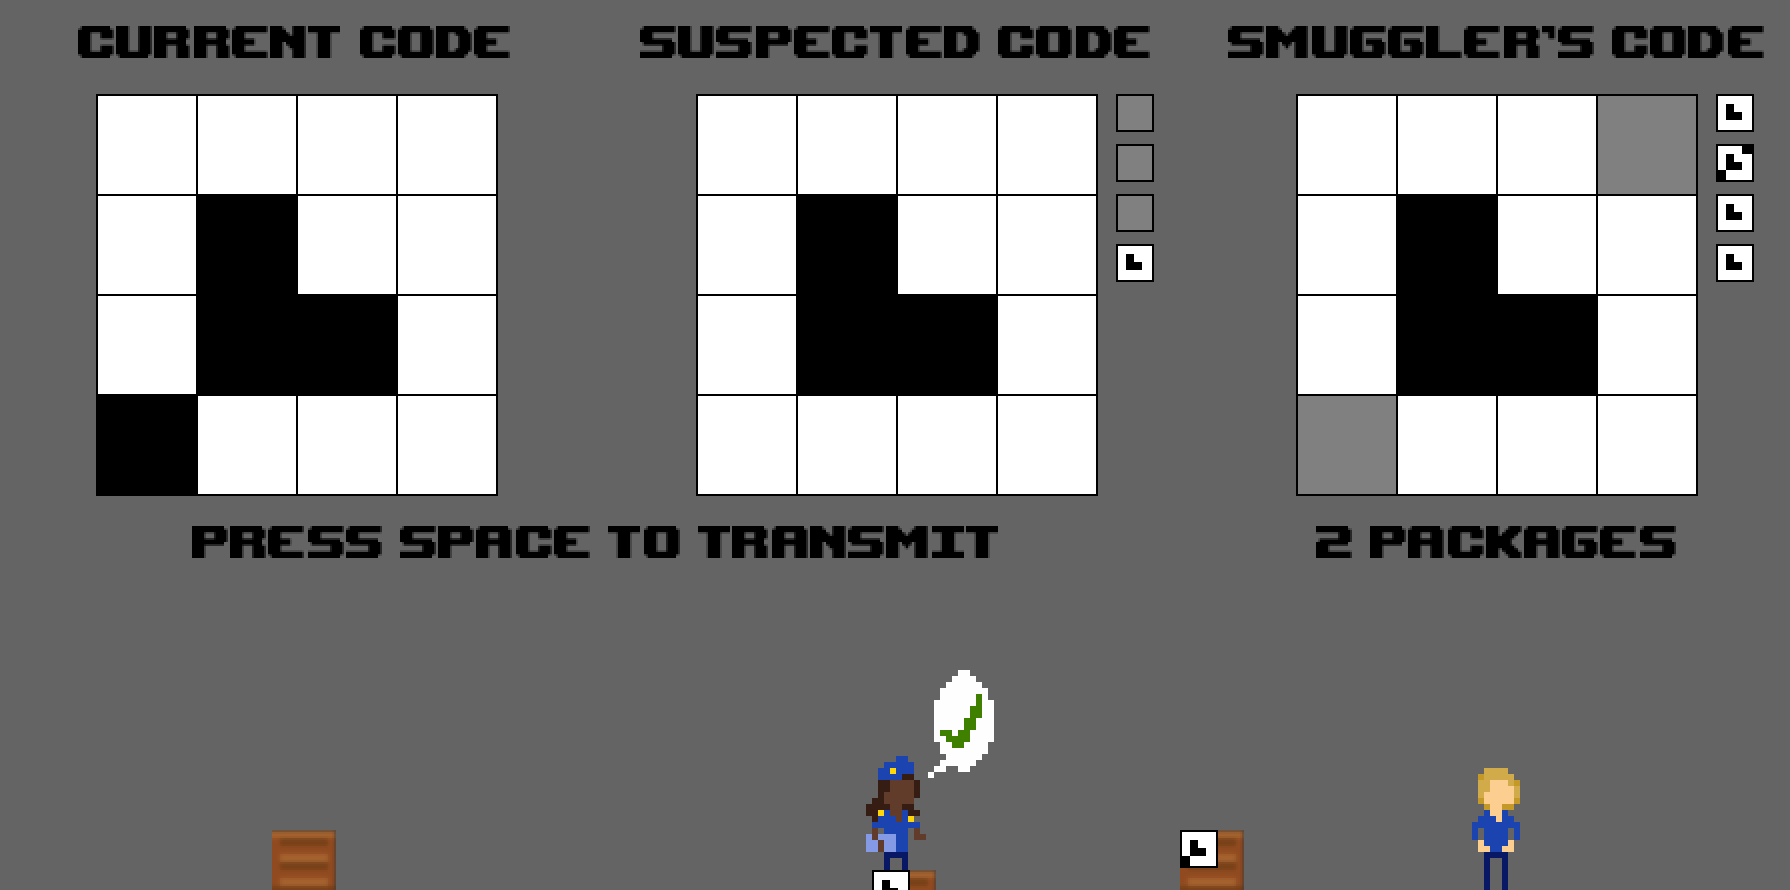
\includegraphics[width=0.5\textwidth]{images/contrabot}
\caption{{\sc Contrabot} interface: player input code on the left; inspector learned code in the middle; smuggler learned code on the right. Agent memories are shown as the set of smaller codes along the right of the larger central codes.}
\label{fig:contrabot}
\end{figure}

{\sc Contrabot}\footnote{\url{https://github.com/gamesbyangelina/contrabot}} (Figure \ref{fig:contrabot}) is a game based on agents that learn abstract codes with gameplay based on understanding, playing against and deceiving a machine learning system.
%
Players act as a smuggler trying to label boxes to communicate with a contact on the other side of a customs checkpoint.
The smuggler is trying to learn the code players use to indicate a box is contraband---but an inspector is randomly checking the same boxes.

The game mechanics revolve around how the smuggler and inspector agents learn to check codes based on codes they have seen.
These agents have two main processes: learning codes and matching new codes against their learned code.
Both agents generalize patterns from example codes---using a form of least general generalization---in their memory to then try to match new codes to these learned patterns.
The inspector has a larger memory than the smuggler and gameplay is based on using reverse-engineering how learning works to take advantage of the smuggler forgetting old patterns more quickly than the inspector.
%
The generalization process is simple, when comparing all codes seen the agents memorize exact matches for black or white tiles and generalizing to gray tiles if a position has been occupied by both colors.
Despite this simplicity the design accommodates many levels of difficulty and risk-reward considerations for players based on the size of the codes used and memory capacities of each agent.

We designed {\sc Contrabot} gameplay around risk-reward considerations for the player.
Both agents start with an empty learned code and empty memory. 
The smuggler learns from the first crate inspected and only retains a memory of the 4 most recent codes inspected. 
The inspector initially only has a random chance to inspect creates; after the inspector chooses to check a crate it begins learning and can either randomly check crates or check crates due to matching.
The inspector has an infinite memory, meaning the inspector will eventually learn a code that matches any new code (this ends the game).
After both agents have learned some code, gameplay revolves around creating codes that the inspector will not check (modulo random checks), but that the partner will check.
The number of crates the player passes to the smuggler serves as a score as the game will eventually end once the inspector learns to match all crates.
While simple, this design highlights how understanding the ways a machine learning algorithm works can be the core part of playing and succeeding at a game: in this case mastering the code learning algorithm to both avoid failure (inspector checks) and achieve success (smuggler checks).


\section{What Did You Do?}
\todo{copy-pasta from FDG paper}

\begin{figure}[tb]
\centering
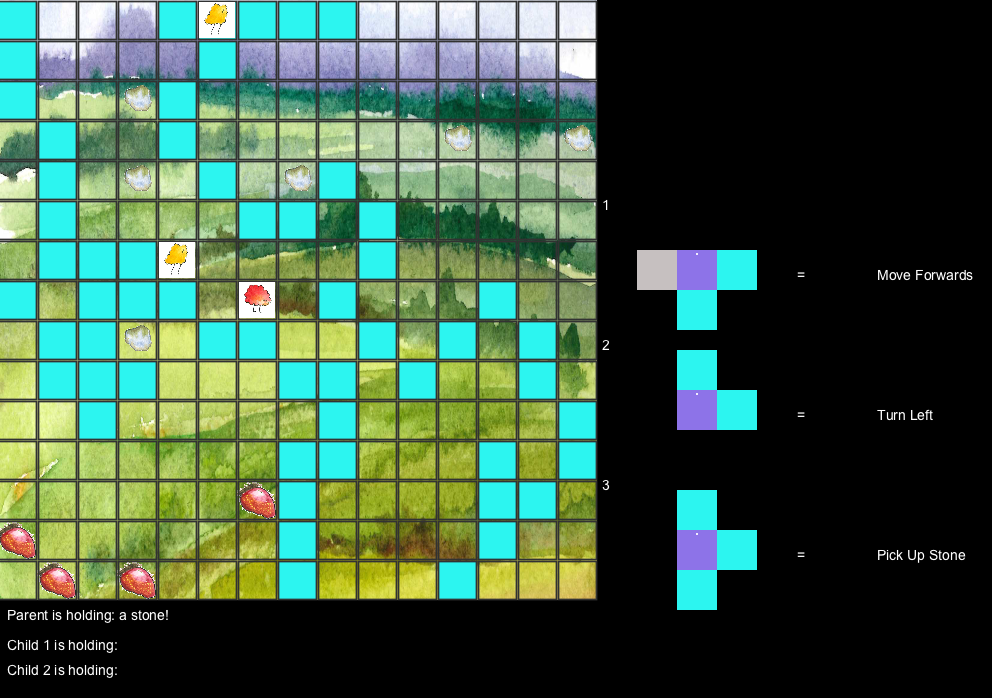
\includegraphics[width=0.5\textwidth]{images/WDYD}
\caption{{\sc What Did You Do?}, a game where the player must supervise non-player characters whose behaviours develop as a result of observing the actions of the player.  The grid pane shows the location of the player and child `shrubs', with the right pane showing the knowledge base the children have learned over time.}
\label{fig:WDYD}
\end{figure}

Game based on training and editing a companion AI agent to complete in-game tasks without the companion failing.
Players control an avatar attempting to raise a computer-controlled child agent in a game environment.
The environment contains a variety of items to manipulate (e.g., stones or foodstuffs) that may be helpful or harmful (e.g., moving stones to stand upon or consuming foodstuffs that may be helpful or poisonous).
Players aim to guide their child through the environment by acting in the world to overcome various obstacles and complete in-world puzzles.
At the same time the child agent applies machine learning techniques to learn to mimic the parent behaviors.
Child learning offers benefits and challenges as the child may help the parent or inadvertently harm itself.
During the game players have access to the memory of the child and may (at a cost) edit what the child has learned.

In What are you doing?2 the player plays as a parent shrub in
charge of protecting and guiding one or several child shrubs. The
challenge the player faces is that the children will not do as they
are told, but instead learn from and mimic the player. This can be
positively lethal for them, however the player possesses a limited
power to edit their minds to unlearn some of the bad habits they've
learned.

https://github.com/gamesbyangelina/whatareyoudoing

The game is turn-based and plays out on a grid as shown in Figure
2. There are five types of entities in the world: the player
character (parent shrub), childshrubs, stones, strawberries, and
ponds. The parent shrub can move in any of the four cardinal
directions, eat or pick up whatever is in the direction it is facing,
or drop something it is carrying. The parent has an energy level
which can be recharged by eating. Child shrubs have mostly the
same actions available, but they have somewhat different effects:
in particular, if the child picks up stone it might be crushed under
its weight, and it will drown if moving into a pool. The energy
levels of the child shrubs are also constantly decreasing. Both
stones and ponds block the way, but stones can be picked up and
moved elsewhere. If a stone is placed into a pond both the pond
and stone disappears, so the tile becomes empty (passable).
Strawberries can be eaten by parents or kids and will increase
energy. As children will rarely seek out strawberries, the parent
can pick up strawberries and drop them on child shrubs so they
eat.

In a pane to the right of the main game area the shared mind of the
children is visualized. Their mind is initially empty, but as the
children watch the parent act, they learn rules. Rules are of the
form "when faced with certain surroundings, perform a certain
action". For example, they could learn a rule that when standing
with a stone to the left and a pond behind, move forward. Or if in
front of a strawberry, pick up. Rules are re-learned every ten
turns, and there is no limit to how many rules can be learned - this
depends only on how many regularities the rule learning
algorithm can find within the recent history of what the parent has
done. The rule learning algorithm is a simple brute force search
for all rules that can be constructed from recent activity; if using
longer action histories or more actions, this would have to be
replaced with an a priori implementation.

The player has the option at any turn to remove one or more rules
from the mind of the children. This, however, costs energy for the
parent, so this possibility must be used sparingly. In order to
replace energy, strawberries can be eaten - but then the same
strawberries cannot be used to feed your children. The reason for
removing rules from the children’s mind is that they would
otherwise hurt themselves, for example drowning in a pond or
picking up a stone and crushing themselves.

Tension is created in the game by scarce resources (energy and
strawberries), but also by the nature of the learning algorithm.
There could be many good courses of action which should be
avoided because your children are watching and could learn the
wrong things. For example, one might want to approach a stone
from the opposite direction than what the shortest path would
suggest, to avoid that the kids see regularities. However, this takes
more time and allows the children to learn more bad behavior in
the meantime. It is also taxing the player's memory to try to
remember what situations the parent has been in recently.
However it is done, there is a clear advantage to reasoning about
the AI, which is reinforced by the visualization of the kids' mind
and the possibility of editing it.

The child shrubs in What Are You Doing? exhibit both the AI as
Trainee pattern and the AI is Editable pattern. In the former case,
player actions are observed by the shrubs, and so the player knows
that by solving problems in the game world they are also giving
new knowledge to the AI agents. In the latter case, pruning
knowledge from the shrubs is a restricted form of editing, in that
knowledge can be explicitly removed from the agents (although
new knowledge cannot be explicitly added, only implicitly
through behaving in a certain way). Because the learned
knowledge is displayed to the player through a visualization of the
rules, the game also exhibits the AI as Visualizer pattern, through
which the player can understand what knowledge has been picked
up by the shrubs, and then edit it appropriately to remove
dangerous behavior.

The game raises interesting problems with presenting machine
learned knowledge to the player. Our method of machine learning
learned partial rules that may not be thought of as ‘knowledge’ to
a human player unfamiliar with machine learning (such as what to
do when a rock is to your left, but not what to do in the general
case of being adjacent to rocks). This also means that editing
knowledge can be exhausting, since there may be multiple cases
that are all undesirable, which need to be manually removed when
to the player they may seem to all stem from the same original
case. The presentation of machine learned knowledge both in
Contrabot and What Are You Doing? presents interesting
possibilities of how to use these technique in future game projects,
and indicates the richness of new ideas to be found in applying
these patterns to new aspects of gameplay.

\cite{smith2012:endlessweb}

\bibliographystyle{abbrv}
\bibliography{../latex/lib}

\end{document}